% ISEF Quad Chart / Visual Summary.
% Spec observed: one landscape page, entire page visible; light background with
% dark text; body text at 18pt minimum (12pt permitted only for figure credits);
% list/bulleted and brief; four EQUAL quadrants each with a single border line;
% title block only as tall as its required elements, Project ID upper right,
% title largest, then name/school/city/state/country. No bibliography, no
% references, no acknowledgements, and the word "abstract" does not appear.
\documentclass[landscape,letterpaper]{article}
\usepackage[margin=0.40in,landscape,letterpaper]{geometry}
\usepackage{amsmath,amssymb,graphicx,booktabs}
\usepackage[T1]{fontenc}
\usepackage{xcolor}
\pagestyle{empty}
\setlength{\fboxsep}{5pt}\setlength{\fboxrule}{0.7pt}
\setlength{\parindent}{0pt}
\graphicspath{{figures/}}

\definecolor{ink}{RGB}{14,32,64}
\definecolor{rule}{RGB}{60,80,115}
\definecolor{panel}{RGB}{247,249,253}

\newcommand{\qhead}[1]{{\fontsize{19}{22}\selectfont\bfseries\color{ink}#1}\\[3pt]}
\newcommand{\bul}{\leavevmode\hbox to 1.1em{\color{rule}\textbullet\hfil}}

% one quadrant: fixed size so all four are equal, single border line
\newlength{\qw}\newlength{\qh}
\setlength{\qw}{4.84in}
\setlength{\qh}{2.98in}
\newcommand{\quadrant}[1]{%
  \fcolorbox{rule}{panel}{\begin{minipage}[t][\qh][t]{\qw}%
    \setlength{\parskip}{3pt}\fontsize{18}{21.5}\selectfont\color{black}%
    \hspace{4pt}\begin{minipage}[t]{\dimexpr\qw-14pt\relax}#1\end{minipage}%
  \end{minipage}}}

\begin{document}
\fontsize{18}{21.5}\selectfont

%% ---------------- title block: only as tall as its required elements
\begin{minipage}[t]{0.80\textwidth}
{\fontsize{20}{23}\selectfont\bfseries\color{ink}
Where Optimal Networks Stop Existing: Certified Spectral Limits of Cyclic Architectures\par}
\vspace{2pt}
{\fontsize{18}{21}\selectfont Aryan Padarthi \quad\textbar\quad
\rule{2.6in}{0.5pt} \ (school, city, state, country)\par}
\end{minipage}%
\hfill
\begin{minipage}[t]{0.19\textwidth}\raggedleft
{\fontsize{18}{21}\selectfont Project ID\\[2pt]\rule{1.5in}{0.5pt}\par}
\end{minipage}

\vspace{3pt}

%% ---------------- quadrants
\begin{tabular}{@{}c@{\hspace{5pt}}c@{}}
\quadrant{%
\qhead{1. Research Question}
\bul Every graph has an \textbf{Ihara zeta function}, so one can state the
\textbf{Riemann Hypothesis} for a graph --- and unlike the classical case it is
\textbf{decidable}: a cubic graph satisfies it exactly when every eigenvalue of
modulus $\ne3$ has modulus $\le2\sqrt2$.

\bul \textbf{Which generalized Petersen graphs satisfy it?} Their spectrum is
known; the question is not asked.
}
&
\quadrant{%
\qhead{2. Methodology / Project Design}
\bul \textbf{Clear the radicals.} Substituting $\pm2\sqrt2$ into the
characteristic polynomial and squaring twice (each an \emph{equivalence}) leaves
one integer polynomial $D_k$ of degree $2k+2$, evaluated on the grid.

\bul \textbf{Read the endpoints.} $D_k(1)=-7$ always; $D_k(-1)=-7$ for odd $k$,
$+9$ for even $k$. Each forbids a band the grid must miss.

\bul \textbf{Certify exactly} in $\mathbb Z[\zeta_m]$.
}
\\[5pt]
\quadrant{%
\qhead{3. Data Analysis \& Results}
\vspace{-6pt}
\begin{center}
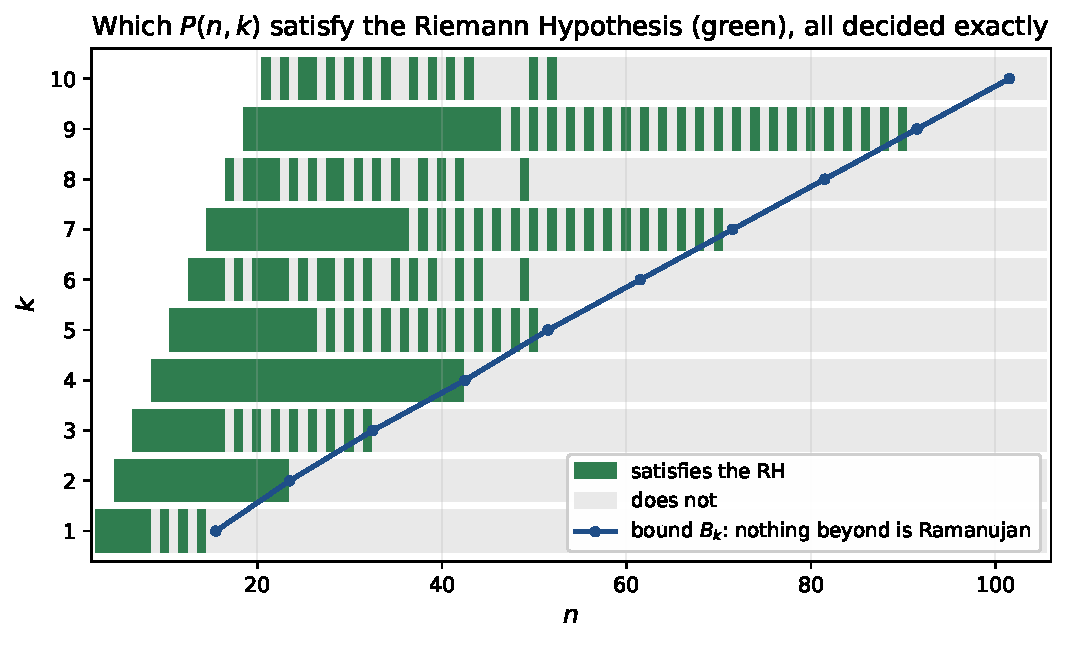
\includegraphics[height=2.05in]{fig_ramclass.pdf}
\end{center}
\vspace{-8pt}
{\fontsize{12}{13.5}\selectfont Figure: author's own work, Python and \TeX,
2026. Green: satisfies the RH. Line: the bound $B_k$ of the finiteness theorem.\par}
}
&
\quadrant{%
\qhead{4. Interpretation \& Conclusions}
\bul \textbf{Only finitely many $n$ per $k$}, and proved for \textbf{every} $k$:
$n\le\pi(2+\sqrt2)\sqrt{k^2+1}$, by AM--GM and $1-\cos\theta\le\theta^2/2$.

\bul \textbf{Parity law:} for odd $k$ an even $n$ lands on an exempt
eigenvalue, so \textbf{bipartiteness helps}; odd $n$ stops at half the bound.

\bul \textbf{Criterion with no $k$ in it:} both factors of $D_k$ collapse to
$Q=4x^2+4y^2-8\sqrt2|xy|+3\ge0$ --- one fixed forbidden set for every $k$.

\bul \textbf{Complete classification}, every $n$ and every $k$: $460$ pairs
($324$ up to isomorphism), $13{,}110$ cases decided exactly, $0$ disagreements.
Dirichlet's theorem bounds $n$ uniformly in $k$; nothing past $k=45$.
}
\end{tabular}

\end{document}
